\section{Determine the optimal edges}

\subsection{Considered detectors}

We have considered seven different detectors:
\begin{itemize}
	\item Simple derivative and thresholding method
	\item Sobel derivative and thresholding with Non-Maximum Suppression (NMS). This method finds edges using the Sobel approximation to the derivative. It returns edges at those points where the gradient of the image is higher than a certain threshold. The NMS takes care of thinning the edges.
	\item Prewitt derivative and thresholding with NMS. Just like Sobel, but using the Prewitt approximation of the derivative instead.
	\item Roberts derivative and thresholding with NMS. Works like Sobel and Prewitt, but using the Roberts approximation of the derivative.
	\item LoG (Laplacian of Gaussians). This method performs the convolution of the image with an approximation of the Laplacian of a Gaussian function. There is also a threshold involved with a similar role like in the previous methods.
	\item Zero-cross method. This method finds edges by looking for zero-crossings after filtering the image with an arbitrary filter. A threshold may be specified.
	\item Canny. The Canny method finds edges by looking for local maxima of the image's gradient. 	The edge function calculates the gradient using the derivative of a Gaussian filter. 	This method uses two thresholds to first detect strong edges and then weak edges connected to the strong edges.
\end{itemize}

The simple derivative detector has been implemented by us as follows:
\begin{subequations}
\begin{equation}
D_x = [-1 \ 1] \quad D_y = [1 \ -1]^T
\end{equation}
\begin{equation}
B_x = I * D_x \quad B_y = I * D_y \quad B^{\circ2} = B_x^{\circ2} + B_y^{\circ2}
\end{equation}
where $|\cdot|^{\circ2}$ denotes the element-wise square of a matrix.
\begin{equation}
I_{edges} = B^{\circ2}_{\geq T^2}
\end{equation}
where the $A_{\geq t}$ denotes a matrix with 1 in each position $(i,j)$ where $a_{ij} \geq t$, and
zero otherwise. Notice that $T$ is the threshold and that we do not perform NMS.
\end{subequations}

We have used the standard MATLAB implementations to test the other methods (available through the \emph{edge} function).

In order to perform our experiments, we have implemented an interface with interactive controls so the user can select the detector and its parameters during runtime \texttt{exercise1.m}. An example of these controls can be seen in figure \ref{fig:simplegui}. There is also a more classical script with the name \texttt{exercise1.m.old}.

\subsection{Comparison of methods}

As to which is the best edge detector, there is no general answer. It highly depends on the application and the evaluation criteria. For our analysis, we consider mainly these four aspects: 
\begin{itemize}
	\item general performance
	\item performance when methods automatically set their own parameters
	\item number of parameters if manual fine tuning is needed
	\item efficiency
\end{itemize}
The last of these qualities could be measured thanks to the experiments in exercise \ref{sec:enhancing}.

The Canny detector is the most sophisticated detector and has a very
good performance for a wide domain of images. It yields very good results when we let the detector
choose automatically the threshold parameters and with the default $\sigma = 1$. The most obvious
drawbacks are that it is the most time-consuming method and that, when the default parameters do not
work good enough, we have to fine-tune three parameters (the high threshold, the low threshold and the $\sigma$ value) for our particular application. Even so, a fixed set of parameters can give
outstanding results for some applications. Results can be seen in figure \ref{fig:im6}. 

\begin{figure}[!hbt]
  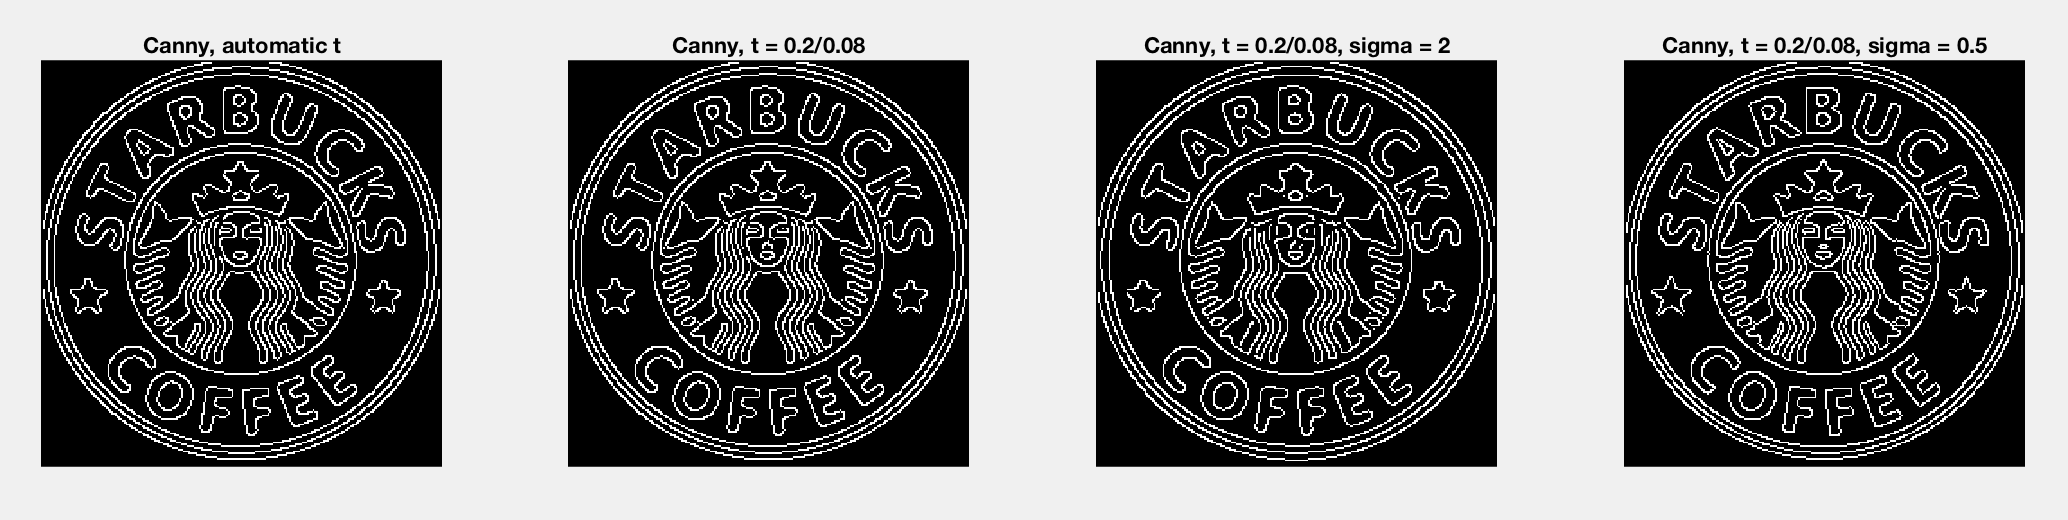
\includegraphics[width=\textwidth]{./img/ex1/im6.png}
  \caption{Results with Canny method}
  \label{fig:im6}
\end{figure}

The Sobel, Prewitt and Roberts detector lead to very similar results. The main difference among them
is how they approximate the derivative. The Roberts detector has the particularity of not being useful
for calculating the horizontal/vertical edges, because it uses approximation of the diagonal
derivatives instead of the derivatives along the main axis. These detectors are quite fast, and in
some cases they give reasonable performance when we let the detector find the threshold automatically.
Usually it is necessary to tweak the threshold to obtain results more akin to our perception of
the edges. An advantage with respect to the Canny detector is that the method takes only one parameter
(if we let the direction of the edges aside). We can see some results in figures \ref{fig:im1},
\ref{fig:im2} and \ref{fig:im3}.

\begin{figure}[!hbt]
  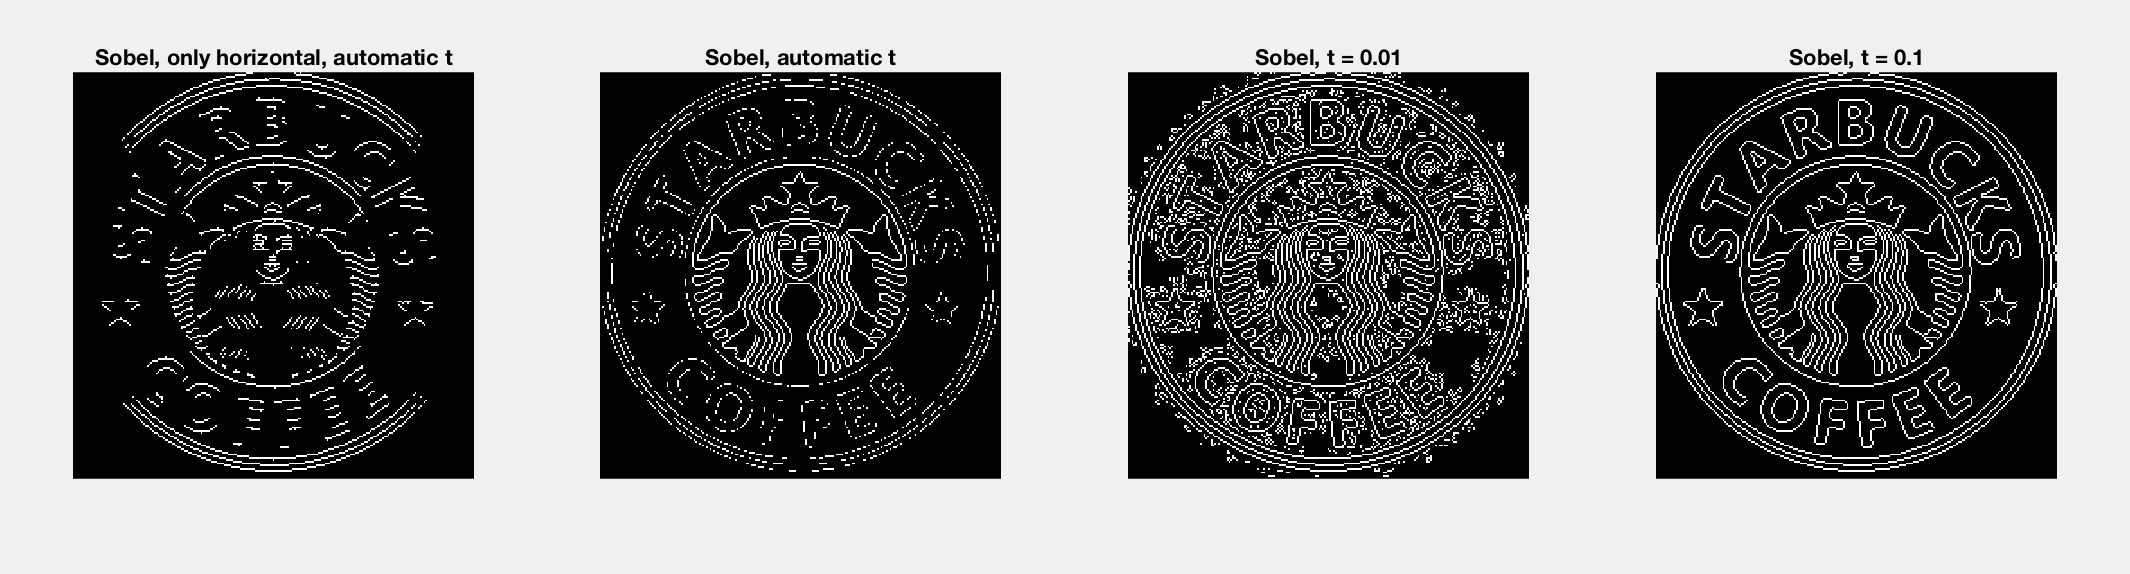
\includegraphics[width=\textwidth]{./img/ex1/im1.png}
  \caption{Results with Sobel method}
  \label{fig:im1}
\end{figure}

\begin{figure}[!hbt]
  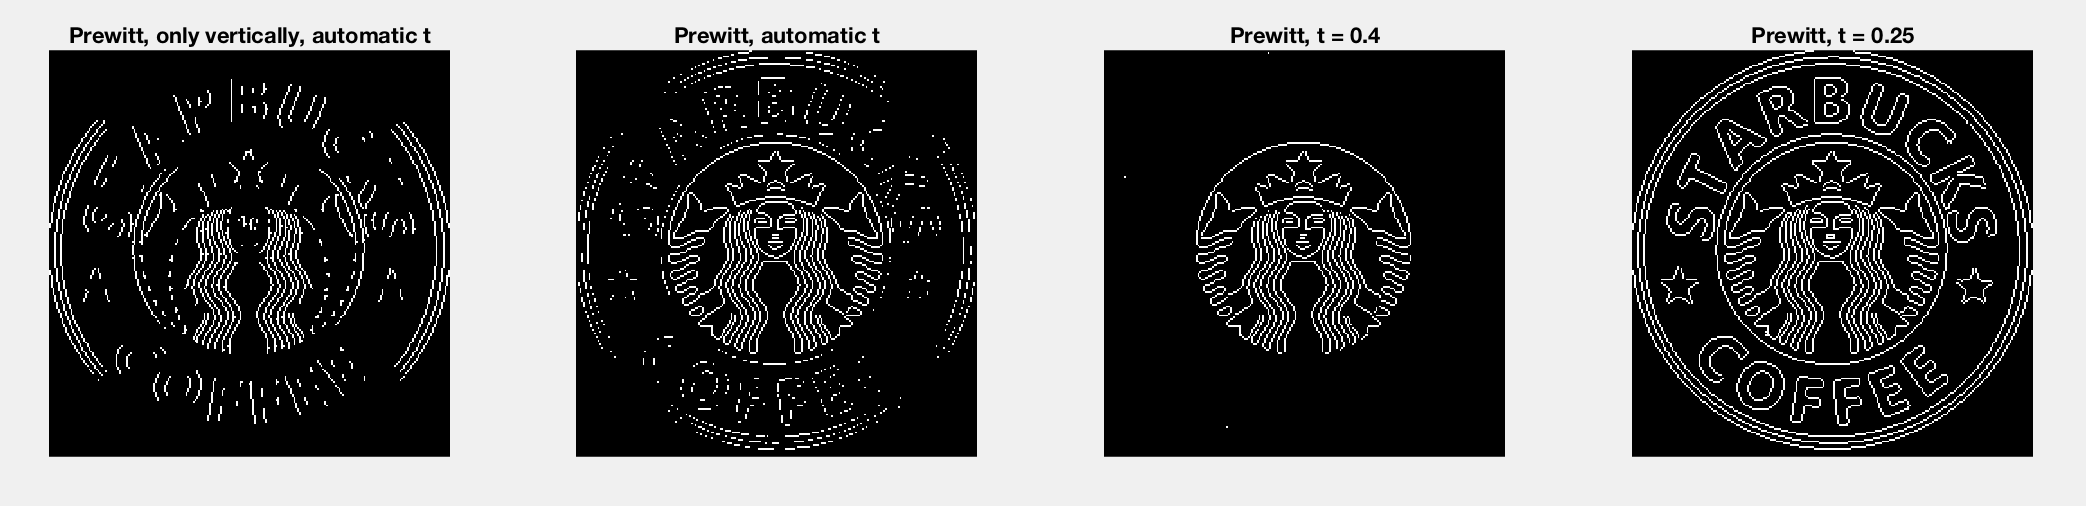
\includegraphics[width=\textwidth]{./img/ex1/im2.png}
  \caption{Results with Prewitt method}
  \label{fig:im2}
\end{figure}

\begin{figure}[!hbt]
  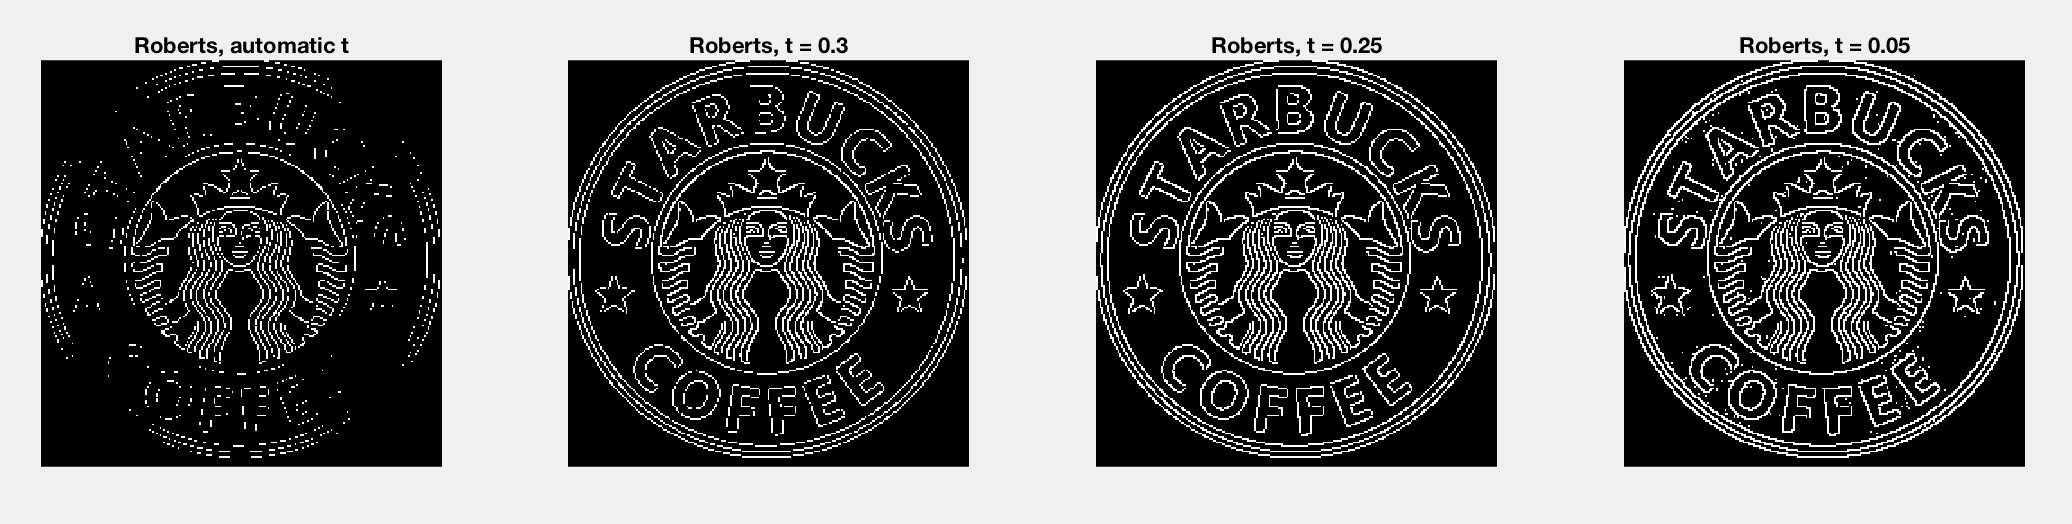
\includegraphics[width=\textwidth]{./img/ex1/im3.png}
  \caption{Results with Roberts method}
  \label{fig:im3}
\end{figure}

The simple derivative detector did not provide any clear advantage over the previous filters neither
in time nor in efficiency. Moreover, we do not perform NMS to thin the edges and it is pretty vulnerable to noise. The only advantage is that it is very simple to implement, even in low-level languages like C or ASM. In practical applications, this is the only reason why this
method might be preferred over any of the previous ones. Much like Sobel, this method takes just
one parameter. It is worth mentioning that we have also implemented a strategy for automatically
selecting the threshold. This automatic threshold selection consists in taking 2 times the
average of $B^{\circ2}$ (i.e. in terms of signal processing, 2 times the \emph{power} of $B$).
Graphical results can be seen in figures \ref{fig:simplegui} and \ref{fig:simpleguinoisy}.

\begin{figure}
	\centering
	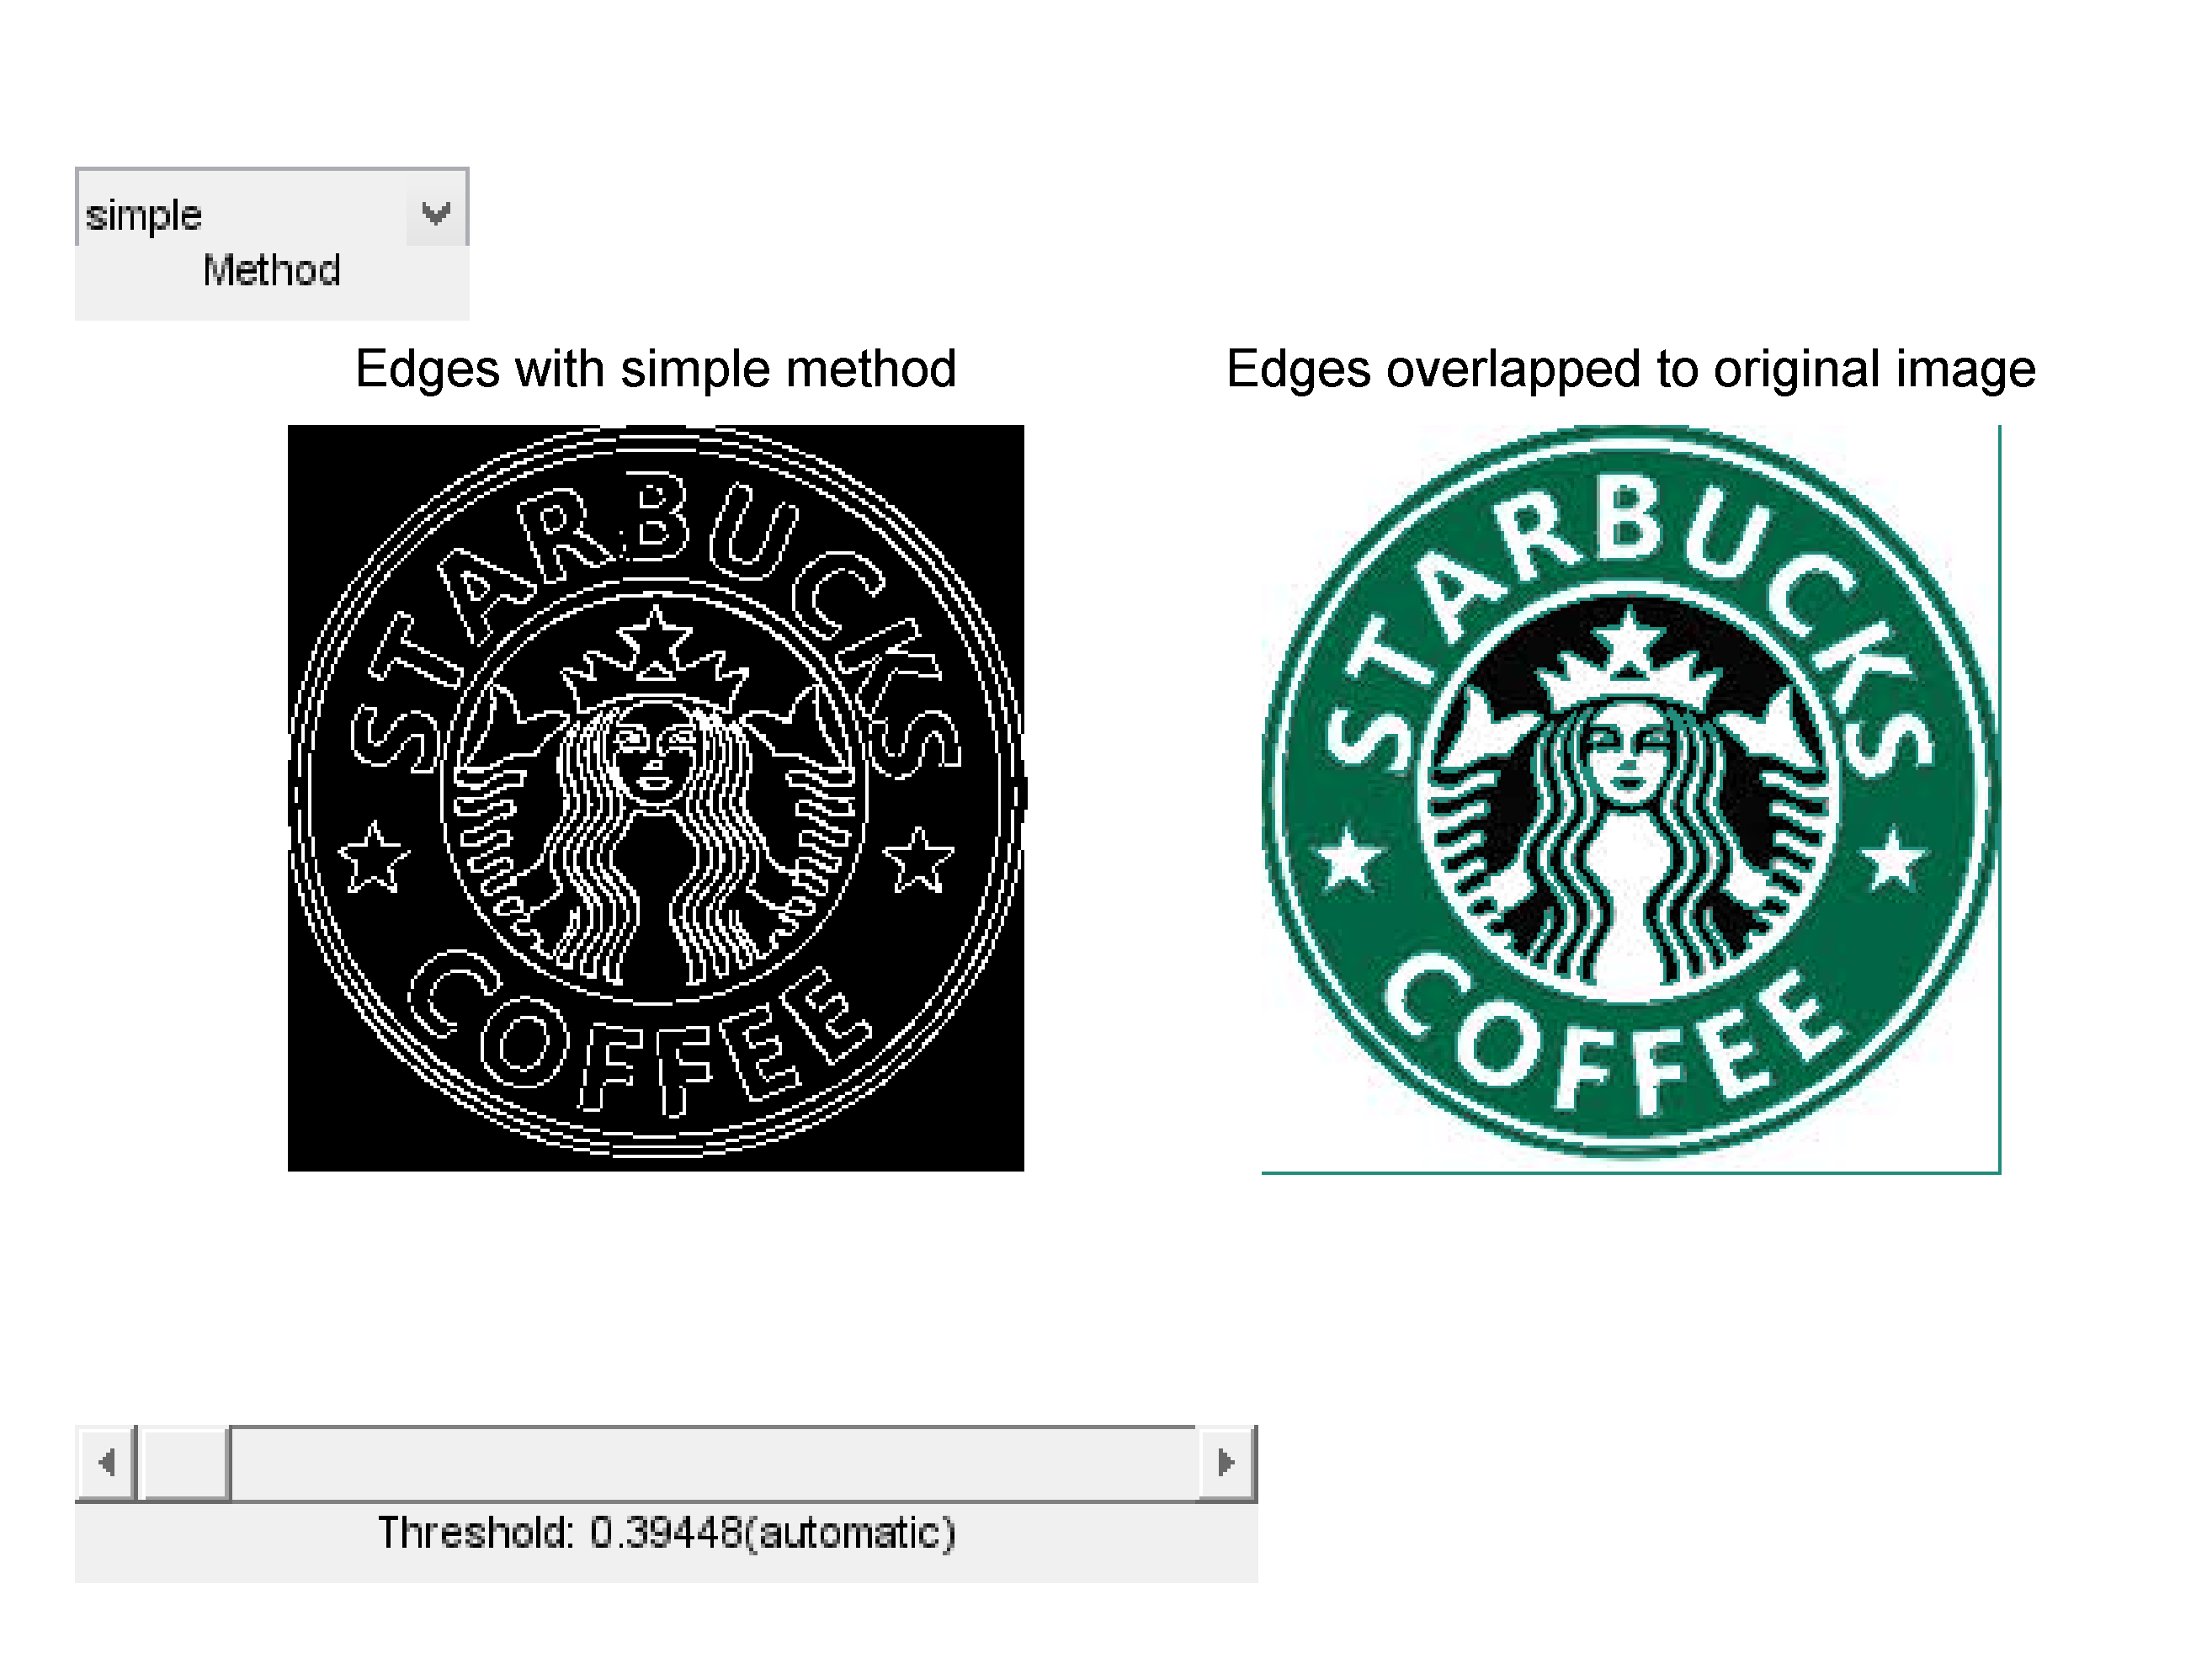
\includegraphics[height=6cm]{./img/ex1/simplegui.png}
	\caption{Simple detector with arbitrary threshold. Observe the thick edges.}
	\label{fig:simplegui}
\end{figure}

\begin{figure}
	\centering
	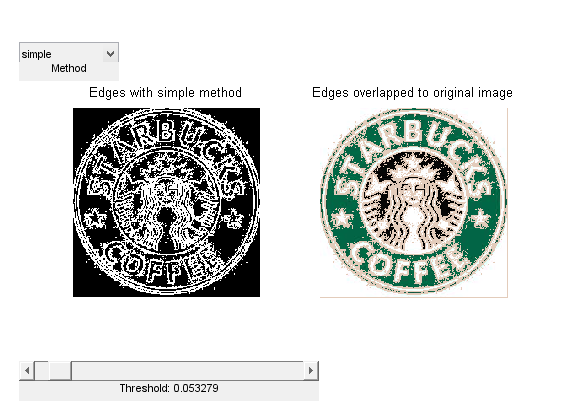
\includegraphics[height=6cm]{./img/ex1/simpleguinoisy.png}
	\caption{Simple detector with arbitrary threshold. Observe the noisy behavior.}
	\label{fig:simpleguinoisy}
\end{figure}

The LoG method provides good results when using the automatic threshold and the default $\sigma$.
However, it has the drawback of being too reactive to changes in the input (i.e. for a fixed
$\sigma$, a small increment of the threshold can be the difference between clearly extracted edges
and a poor edge selection). In terms of efficiency, it is between the Sobel and the Canny detector.
In case that the automatic selection of the threshold and the default $\sigma$ are not good enough,
there are two parameters to tune, which is also between the Sobel and the Canny method. See some
graphical examples of this edge detector in figure \ref{fig:im4}.

\begin{figure}[!hbt]
  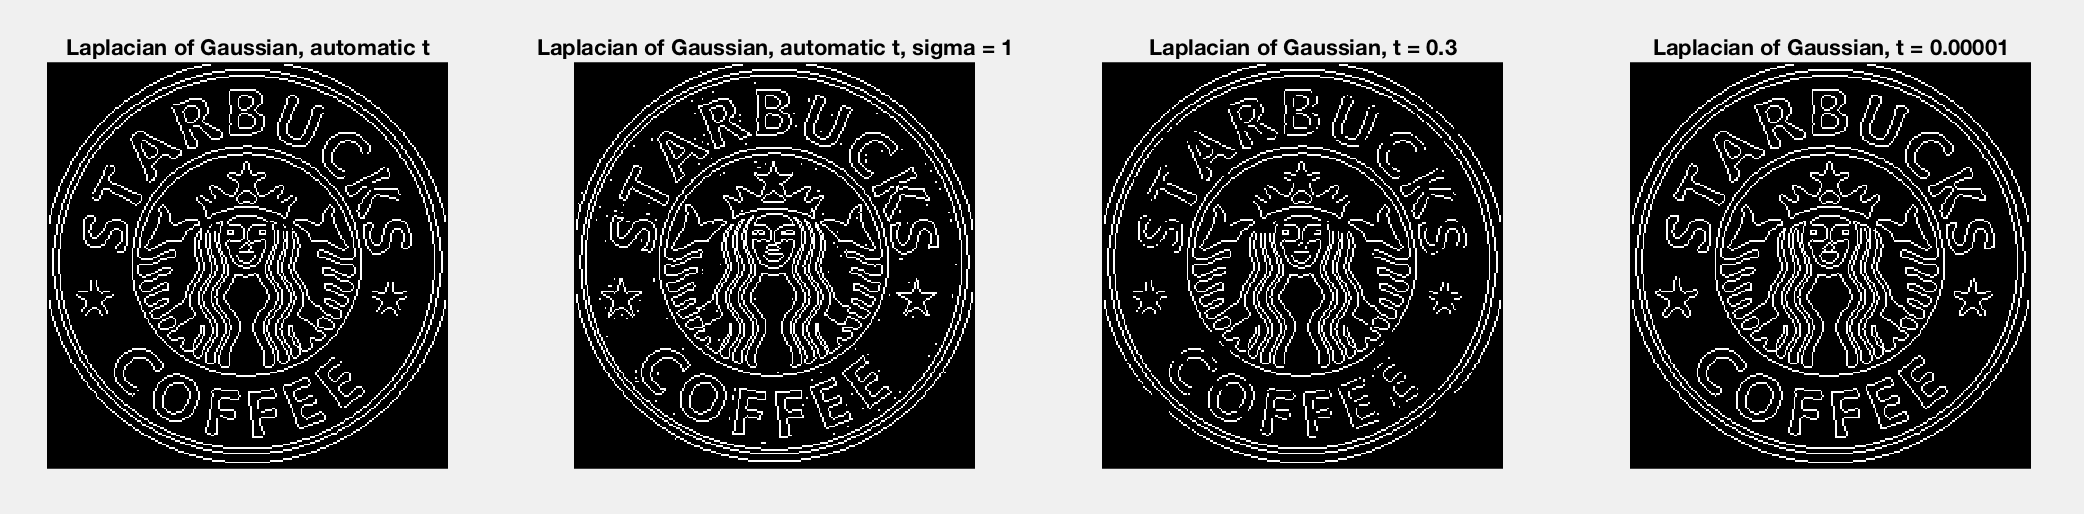
\includegraphics[width=\textwidth]{./img/ex1/im4.png}
  \caption{Results with Laplacian of Gaussian}
  \label{fig:im4}
\end{figure}

Lastly we have the zero-cross method. In our experiments it had a performance very similar to that of
the LoG method (with less abrupt differences when slightly changing the parameters). Also like LoG,
its execution time was between Sobel and Canny. The main particularity of this method is that
we get to choose the filter it applies to the image before computing the edges, so the number of
parameters actually depends upon the filter we choose. We have chosen a Gaussian kernel with
variable $\sigma$ and a kernel size of at least 5 times this $\sigma$, so all in all the method
has two parameters (the threshold and the $\sigma$). We can see some results in figure \ref{fig:im5}.

\begin{figure}[!hbt]
  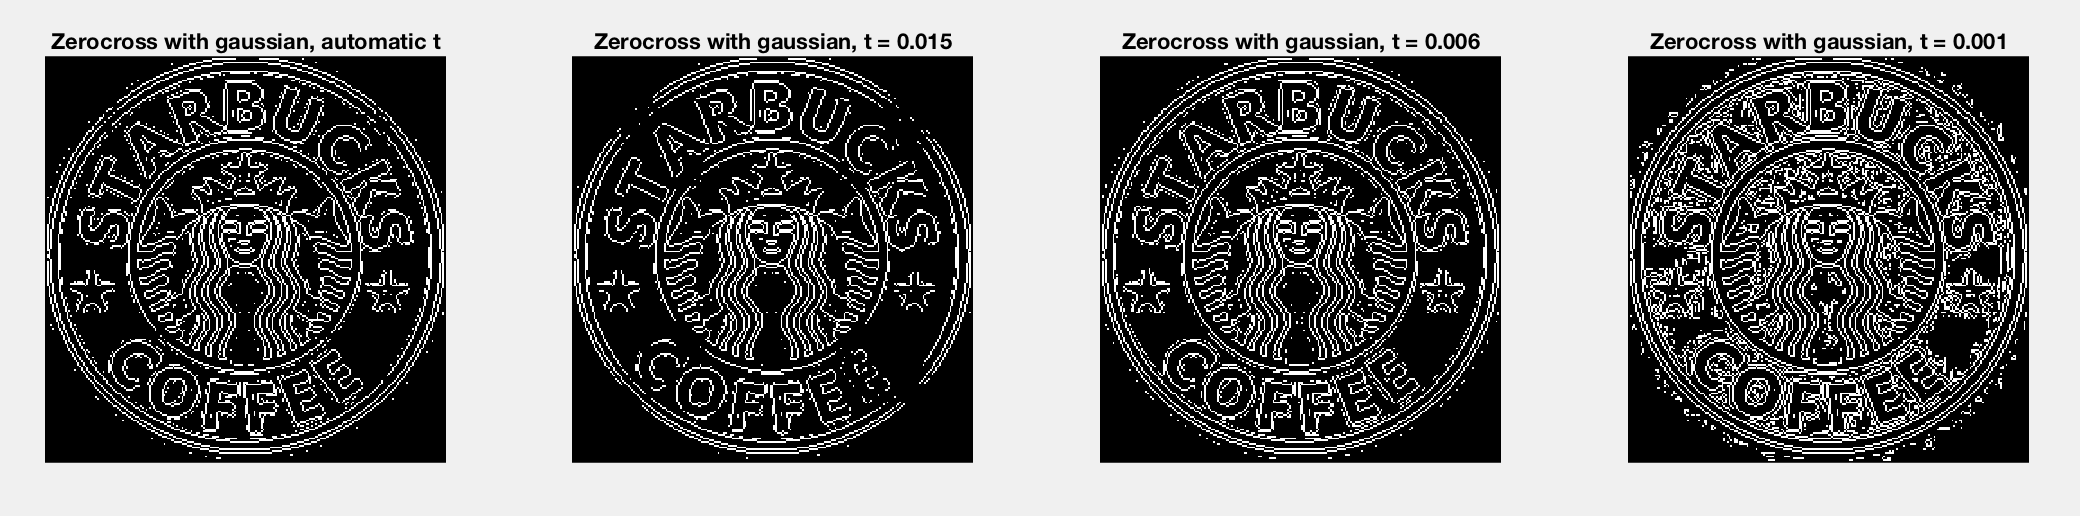
\includegraphics[width=\textwidth]{./img/ex1/im5.png}
  \caption{Results with Zerocross method}
  \label{fig:im5}
\end{figure}

\subsection{Selecting a detector and tuning its parameters}

For this section we assume, based on the previous points, that the Canny detector has the potential
to be the best detector provided that the application allows to tweak its parameters. The edges of the
\emph{Starbucks} logo can be detected almost perfectly with the automatic threshold and $\sigma = 1$,
as it is shown in figure \ref{fig:cannystarbucks}.

\begin{figure}[!hbt]
  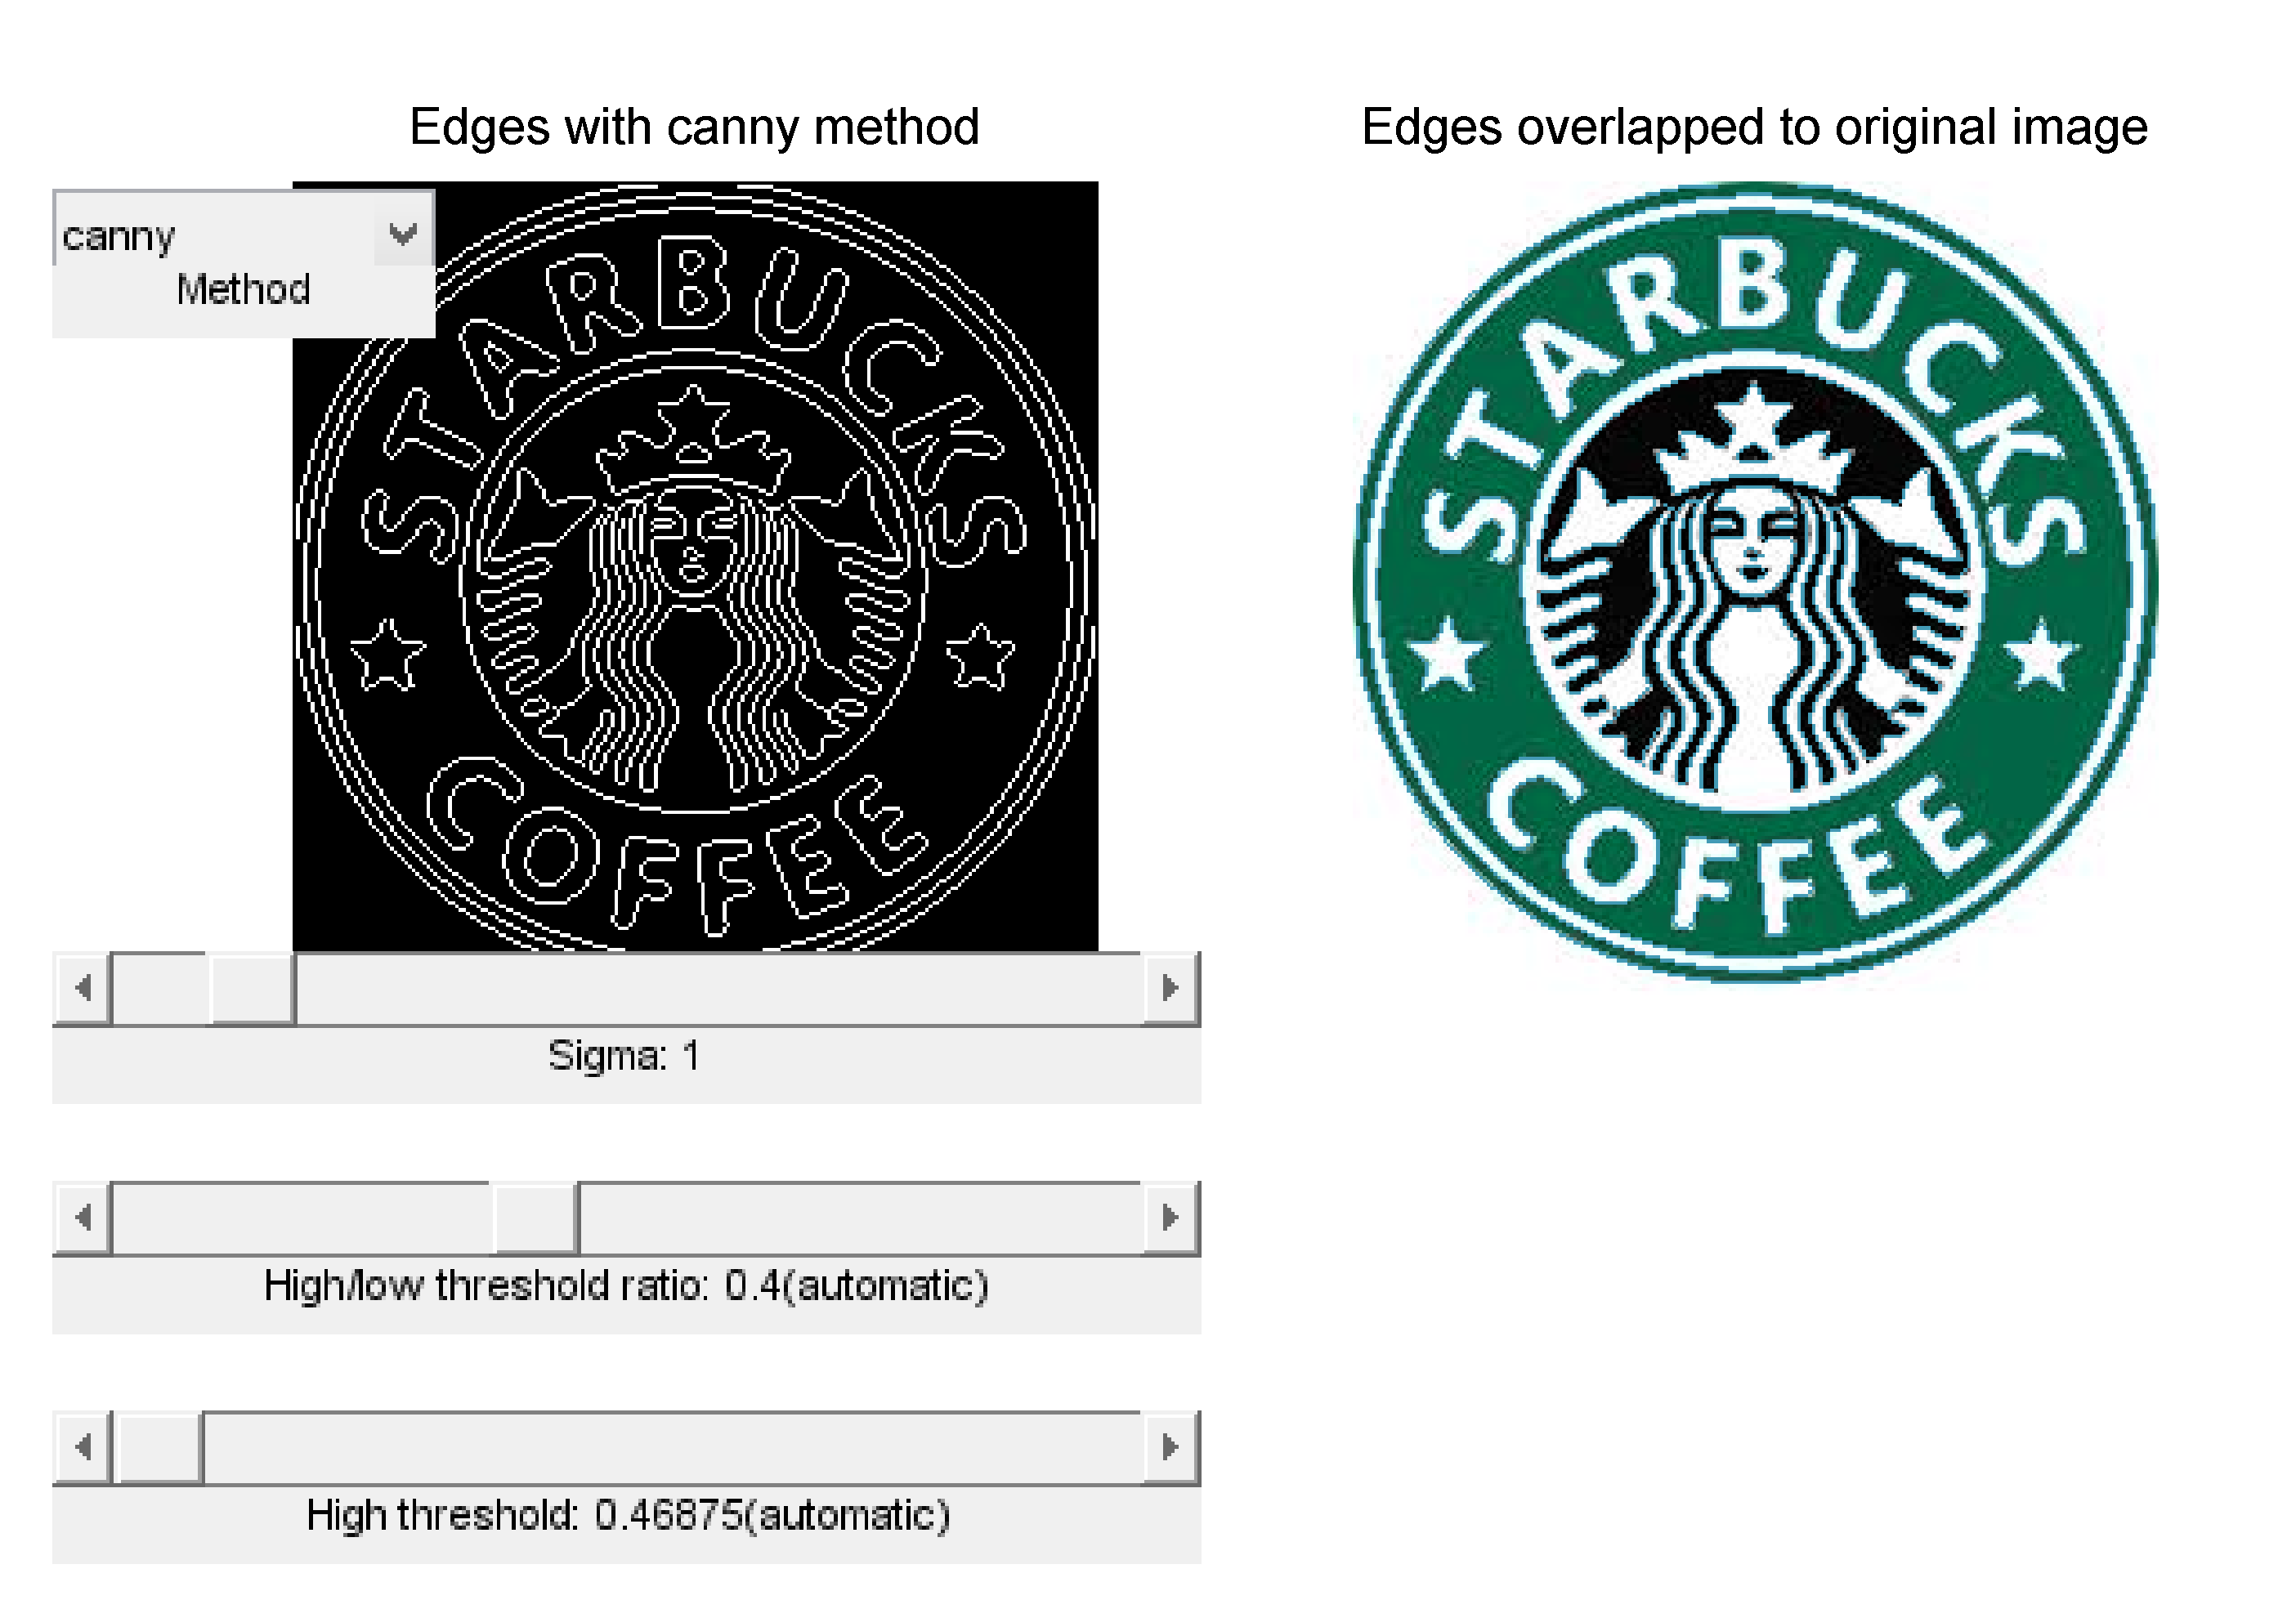
\includegraphics[width=\textwidth]{./img/ex1/canny_gui_starbucks_opt.png}
  \caption{Selected parameters for extracting the edges from the Starbucks logo with Canny}
  \label{fig:cannystarbucks}
\end{figure}

However, if we try to extract the edges of another image with the same parameters
(i.e. using the same thresholds), we obtain what we can see in figure
\ref{fig:cannydoulphinsamethreshold}.

\begin{figure}[!hbt]
  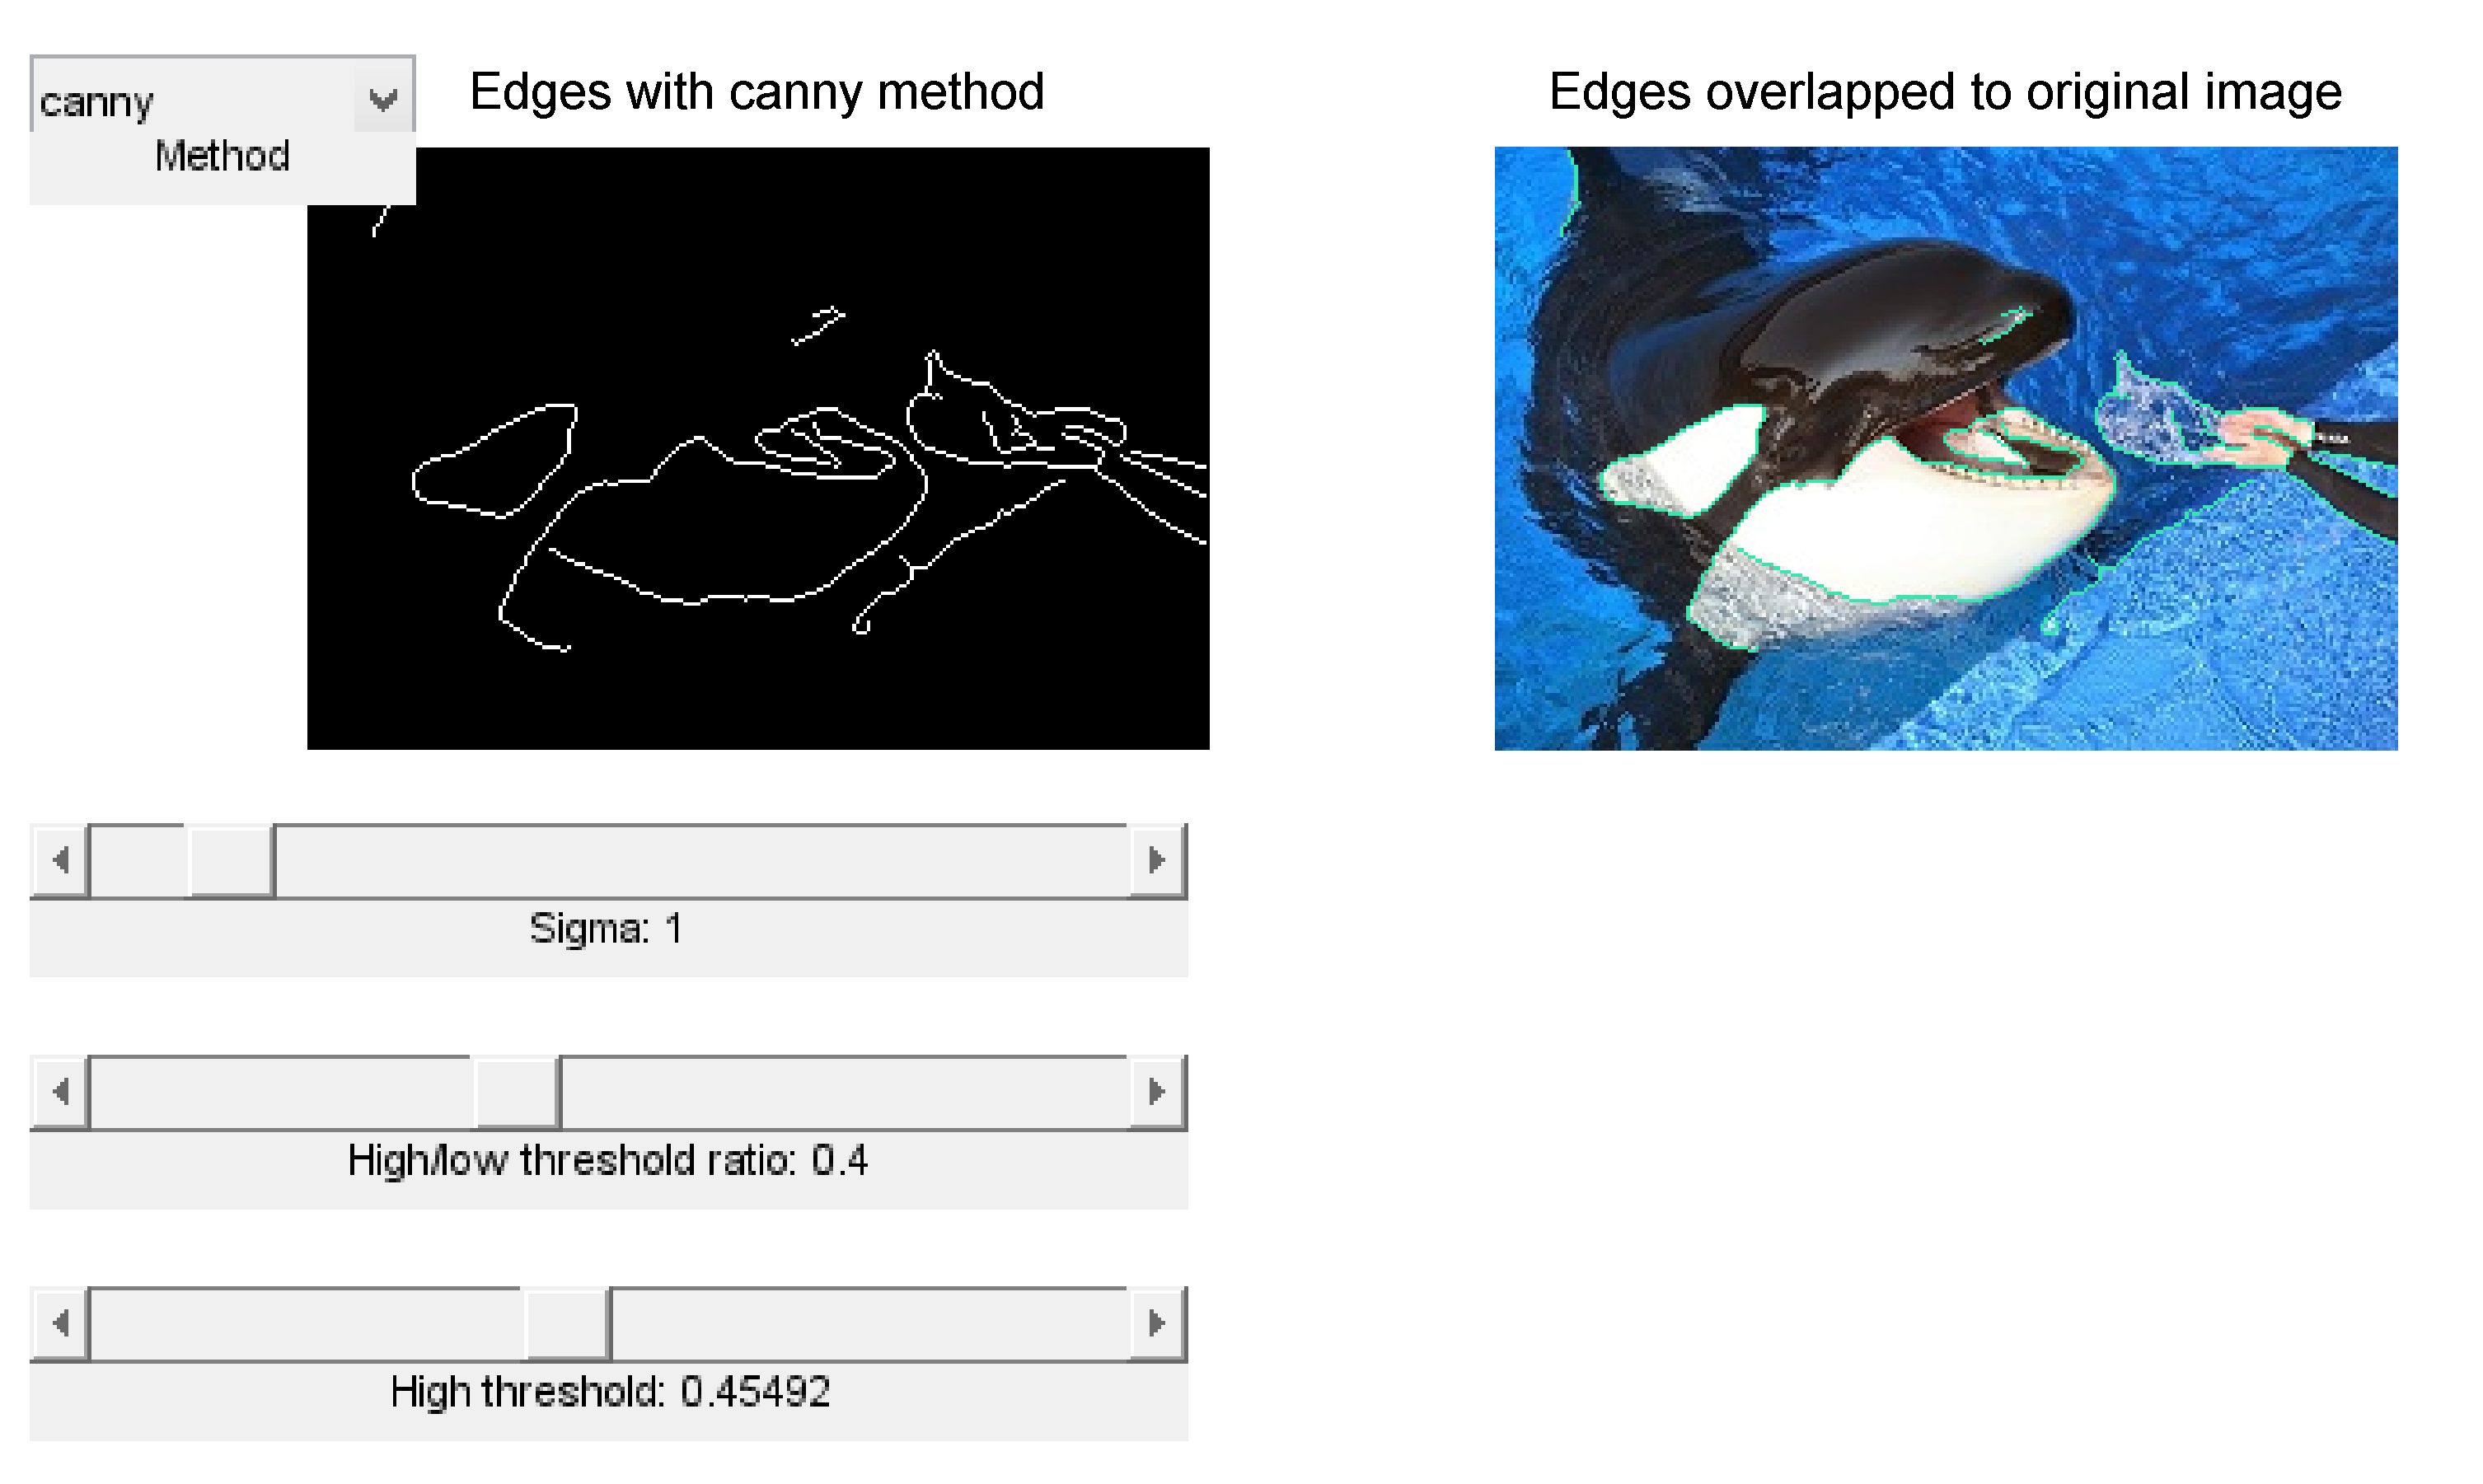
\includegraphics[width=\textwidth]{./img/ex1/canny_doulphin_045.png}
  \caption[Extraction of the edges from \texttt{doulphin.jpg}]
	{Extraction of the edges from \texttt{doulphin.jpg}.
	Observe that the threshold is approximately the same than the used for the edge extraction in
	the Starbucks logo. There are only a few visible edges.}
  \label{fig:cannydoulphinsamethreshold}
\end{figure}

For this same image, if we let the detector choose the threshold automatically,
we obtain the edges in figure \ref{fig:cannydoulphinautomatic}. In this case,
the automatic threshold gives a reasonable result.

\begin{figure}[!hbt]
  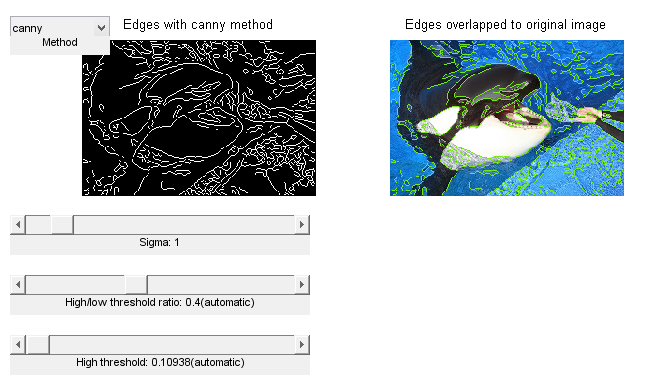
\includegraphics[width=\textwidth]{./img/ex1/canny_doulphin_auto.png}
  \caption[Extraction of the edges from \texttt{doulphin.jpg} using automatic thresholds]
	{Extraction of the edges from \texttt{doulphin.jpg} using automatic thresholds.
	The quality is reasonable. However, we might prefer a less cluttered image.}
  \label{fig:cannydoulphinautomatic}
\end{figure}

Even so, we might prefer fewer and simpler edges. For this, we need to
manually tune the parameters of the Canny detector. Modifying both the
high threshold and the $\sigma$ value, we have obtained the edges of figure
\ref{fig:cannydoulphinselected}, which is arguably the best of the three results
we have shown so far for this image.

\begin{figure}[!hbt]
  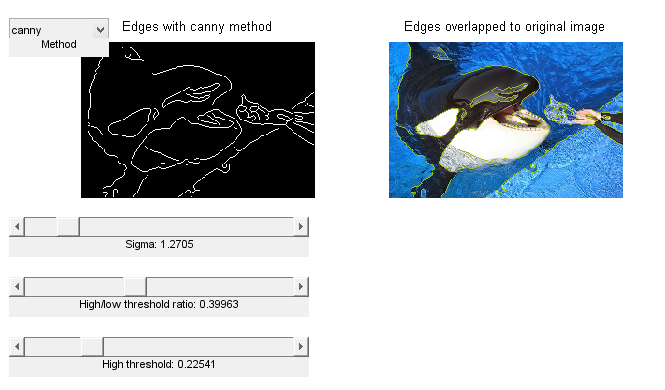
\includegraphics[width=\textwidth]{./img/ex1/canny_doulphin_best.png}
  \caption{Selected parameters for extracting the edges from \texttt{doulphin.jpg} logo with Canny}
  \label{fig:cannydoulphinselected}
\end{figure}

This leads to the conclusion that there does not exist an universal set of
parameters that yield good results for every image. In many cases, to achieve
optimal results we would need to manually tweak the parameters.

We could also need a highly adaptable edge detector for many images
(for example, to extract the edges from a video). In such circumstance,
it is reasonable to let the detector choose automatically the threshold
parameters and to choose the $\sigma$ according to the resolution. Alternatively,
we could set a fixed set of parameters if we believe that they will be good
enough for our particular application.

Although for simplicity we have detailed here just the Canny detector, our
experiments have lead to the same conclusion for the other methods as well.
